\documentclass[problem]{mcs}

\begin{pcomments}
  \pcomment{FP_structural_induction}
  \pcomment{from: Megumi F09}
\end{pcomments}

\pkeywords{
  planar embedding
  structural induction
}

%%%%%%%%%%%%%%%%%%%%%%%%%%%%%%%%%%%%%%%%%%%%%%%%%%%%%%%%%%%%%%%%%%%%%
% Problem starts here
%%%%%%%%%%%%%%%%%%%%%%%%%%%%%%%%%%%%%%%%%%%%%%%%%%%%%%%%%%%%%%%%%%%%%

\begin{problem}  \textbf{Structural Induction}

Consider the following alternative definition of a planar embedding. 

\fbox{\
\begin{minipage}[t]{6.5in}
\vspace{.1in}
\begin{definition*}
A \term{planar embedding} of a 
%\emph{connected} 
graph consists of 
a nonempty set of \emph{sets of discrete faces}.  Planar embeddings are defined recursively as follows:

\vspace{.1in}
\textbf{Base cases:}
If $G$ is a graph consisting of a single vertex,
$v$, then a planar embedding of $G$ has one discrete face, namely the
length zero cycle, $v$.

\vspace{.1in}
\textbf{Constructor Case:}
(split a face) Suppose $G$ is a
graph with a planar embedding, and suppose $a$ and $b$ are
distinct, nonadjacent vertices of $G$ that appear on some discrete face,
$\gamma$, of the planar embedding.  That is, $\gamma$ is a cycle of the form
\[
a \dots b \cdots a.
\]
Then the graph obtained by adding the edge $\edge{a}{b}$ to the edges of
$G$ has a planar embedding with the same discrete faces as $G$, except
that face $\gamma$ is replaced by the two discrete
faces
%\footnote{\label{C} There is one exception to this rule.  If $G$ is a
%line graph beginning with $a$ and ending with $b$, then the cycles into
%which $\gamma$ splits are actually the same.  That's because adding edge
%$\edge{a}{b}$ creates a simple cycle graph, $C_n$, that divides the plane
%into an ``inner'' and an ``outer'' region with the same border.  In order
%to maintain the correspondence between continuous faces and discrete
%faces, we have to allow two ``copies'' of this same cycle to count as
%discrete faces.  But since this is the only situation in which two faces
%are actually the same cycle, this exception is better explained in a
%footnote than mentioned explicitly in the definition.}
\[
a\dots ba\quad \text{ and } \quad ab\cdots a, 
\]
%as illustrated in Figure~\ref{fig:face-splitting}.

%\begin{figure}[h]
%\centering 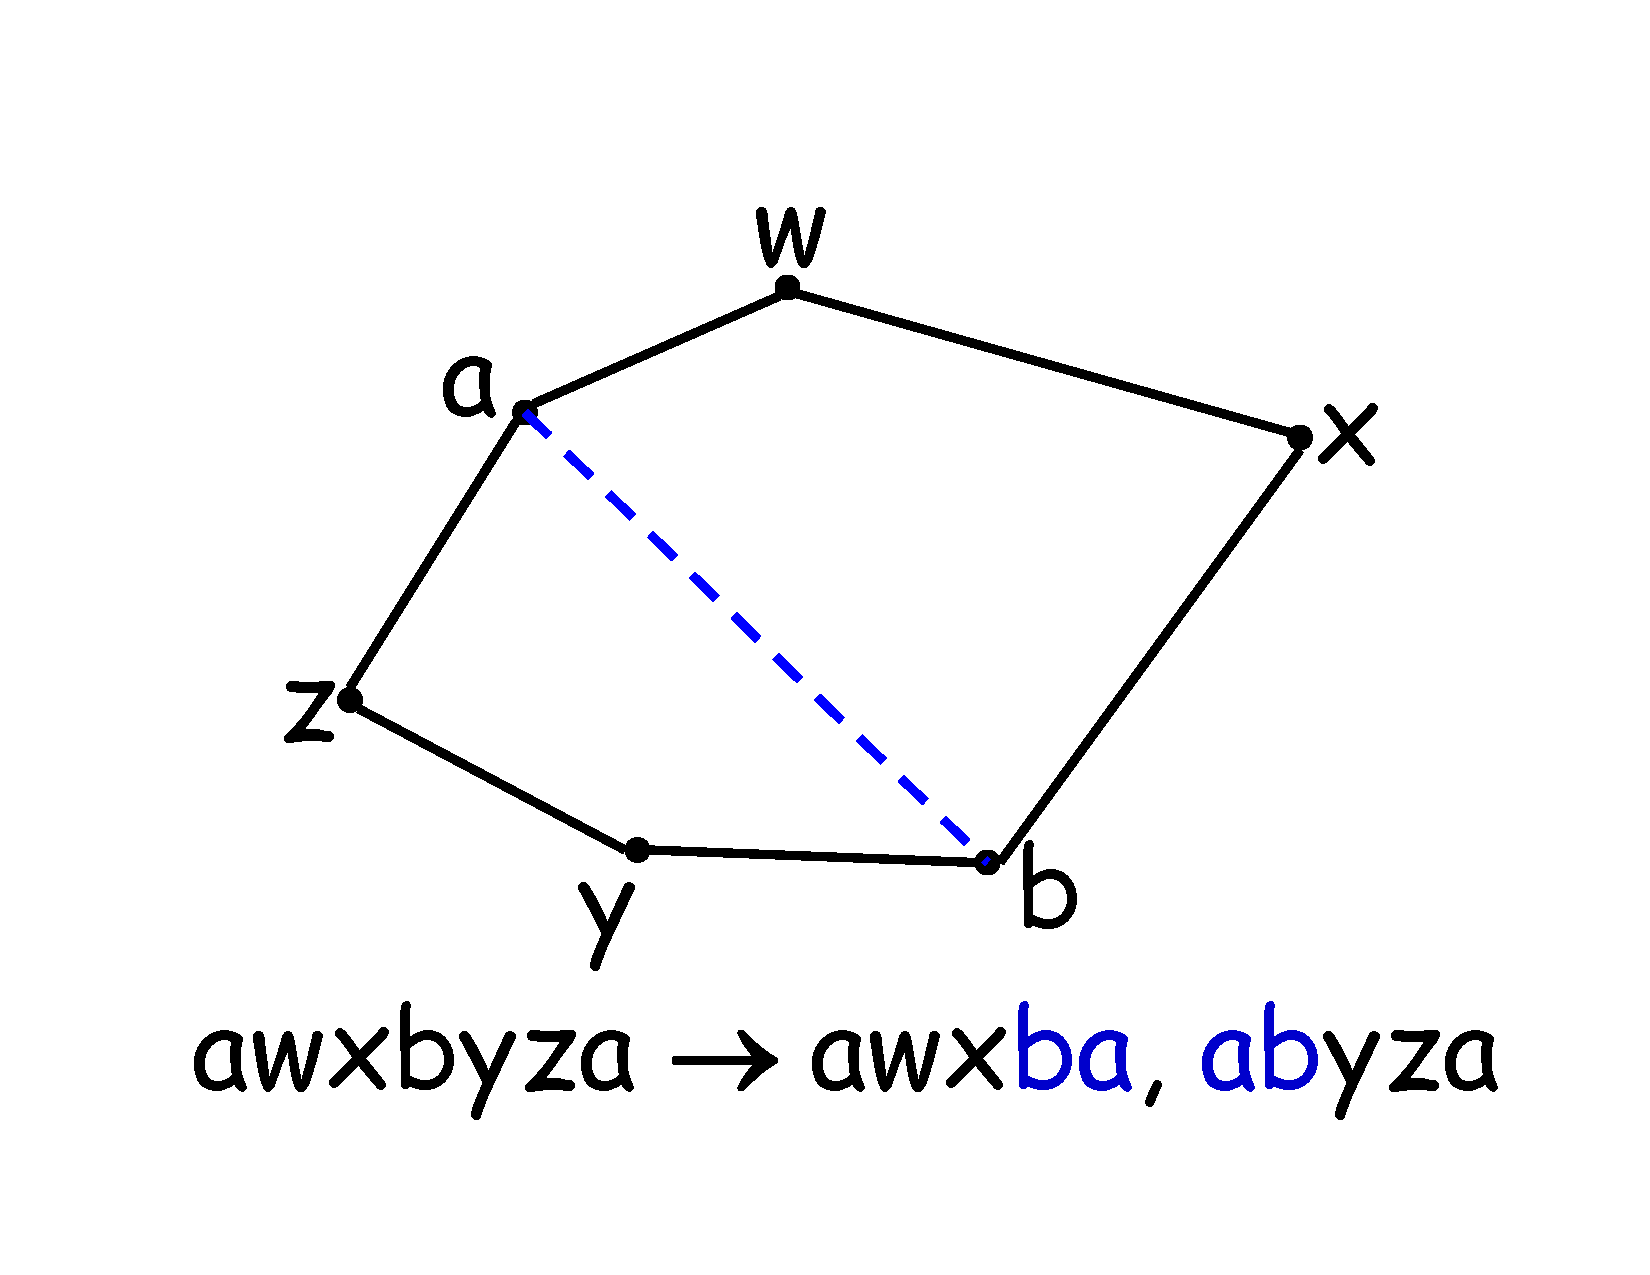
\includegraphics[height=2.5in]{figures/split-a-face}
%\caption{The Split a Face Case.}
%\label{fig:face-splitting}
%\end{figure}

\textbf{Constructor Case:} (add a bridge) Suppose $G$ and $H$ are
graphs with planar embeddings and disjoint sets of vertices.
Let $a$ be a vertex on a discrete face, $\gamma$, in the embedding of
$G$.  That is, $\gamma$ is of the form
\[
a\dots a.
\]
Similarly, let $b$ be a vertex on a discrete face, $\delta$, in the
embedding of $H$, so $\delta$ is of the form
\[
b\cdots b.
\]
Then the graph obtained by connecting $G$ and $H$ with a new edge,
$\edge{a}{b}$, has a planar embedding whose discrete faces are the union of
the discrete faces of $G$ and $H$, except that faces $\gamma$ and $\delta$
are replaced by one new face
\[
a\dots ab\cdots ba.
\]
%This is illustrated in Figure~\ref{fig:add-bridge}, where the faces of
%$G$ and $H$ are:
%\[
%G: \set{\texttt{axyza},\ \texttt{axya},\ \texttt{ayza}}
%    \qquad H: \set{\texttt{btuvwb},\ \texttt{btvwb},\ \texttt{tuvt}},
%\]
%and after adding the bridge $\edge{\texttt{a}}{\texttt{b}}$, there is a
%single connected graph with faces
%\[
%\set{\texttt{axyz{\color{blue}ab}tuvw{\color{blue}ba}},\ 
%         \texttt{axya},\ \texttt{ayza},\ \texttt{btvwb},\ \texttt{tuvt}}.
%\]
%\begin{figure}[h]
%\centering 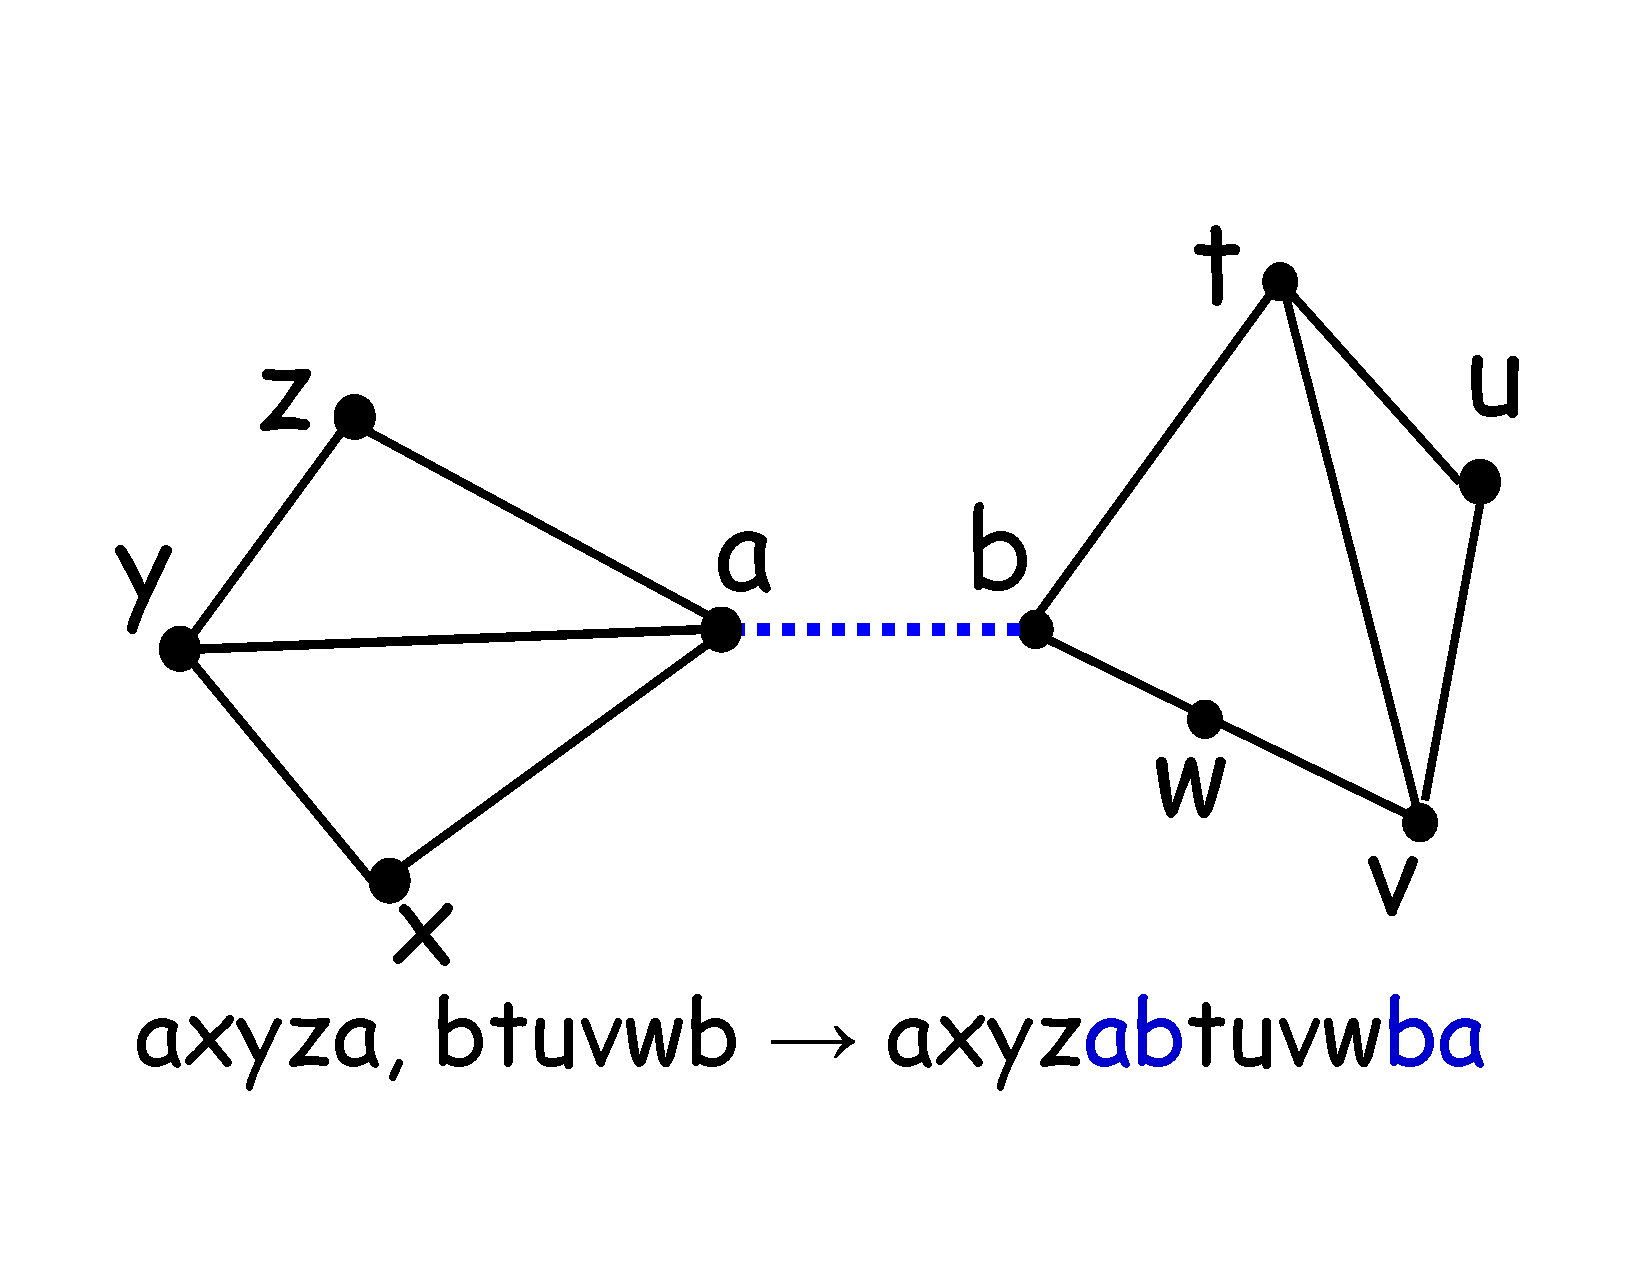
\includegraphics[height=3in]{figures/add-bridge}
%\caption{The Add Bridge Case.}
%\label{fig:add-bridge}
%\end{figure}

An arbitrary graph is \term{planar} iff each of it
has a planar embedding.

\end{definition*}
\end{minipage}}

\examspace[0.1in]

You are asked to prove by structural induction that $v-e+f-2c = 0$, where $v$ is the number of vertices, $e$ is the number of edges, $f$ is the number of faces, and $c$ is the number of connected components.  

\inhandout{\instatements{\newpage}}
\bparts
\ppart Prove the base case of the structural induction.

\begin{solution}
\begin{proof}
TBA
\end{solution}

\examspace[2 in]

\ppart Prove the constructor cases of the structural induction.

\begin{solution}
\begin{proof}
TBA
%  Assuming $f,g$ are rational functions of $x$ for which $P(f)$ and $P(g)$
%  both hold, we must prove $P(h)$ where

%\textbf{Case $h= f + g$}:  In this case,
%\[
%h^{\prime} = f^{\prime} + g^{\prime},
%\]
%and since $f^{\prime}$ and $g^{\prime}$ are rational functions of $x$ by
%hypothesis, so is their sum by the constructor rules, which proves $P(h)$.

%\textbf{Case $h= f \cdot g$}:

%The Product Rule of derivatives states that:
%\begin{equation}\label{fgderiv}
%h^{\prime} =  f^{\prime} \cdot g + f \cdot g^{\prime},
%\end{equation}
%and since $f, f^{\prime}, g, g^{\prime}$ are rational functions of $x$ by
%hypothesis, so is the right hand side of~\eqref{fgderiv} by the
%constructor rules, which proves $P(h)$.

%\textbf{Case $h= \dfrac{1}{f}$}:

%The Chain Rule gives: 
%\begin{equation}\label{1/fderiv}
%h^{\prime} = \frac{-1}{f^2} \cdot f^{\prime},
%\end{equation}
%and since $f$ and $f^{\prime}$ are rational by hypothesis, so is the right
%hand side of~\eqref{1/fderiv} by the constructor rules, which proves
%$P(h)$.

%We have shown that the induction hypothesis holds in all Constructor cases.
%This completes the proof by structural induction.
\end{proof}
\end{solution}

\eparts
\end{problem}


%%%%%%%%%%%%%%%%%%%%%%%%%%%%%%%%%%%%%%%%%%%%%%%%%%%%%%%%%%%%%%%%%%%%%
% Problem ends here
%%%%%%%%%%%%%%%%%%%%%%%%%%%%%%%%%%%%%%%%%%%%%%%%%%%%%%%%%%%%%%%%%%%%%